
Memory allocation in the VM is extremely important because there is a need to
repeatedly allocate and deallocate logical facts. Logical facts tend to be small
memory objects since they are composed of two pointers (16 B) plus a variable
number of arguments (8 B each), which may lead to fragmentation if allocation is
not done carefully.  Moreover, since the VM is multithreaded, allocation also
needs to be scalable, therefore using the standard \code{malloc} facility
provided by the POSIX standard may not be the best idea since each operating
system uses a different implementation that may or may not scale well in
multithreaded environments.

\begin{figure}[ht]
   \begin{center}
      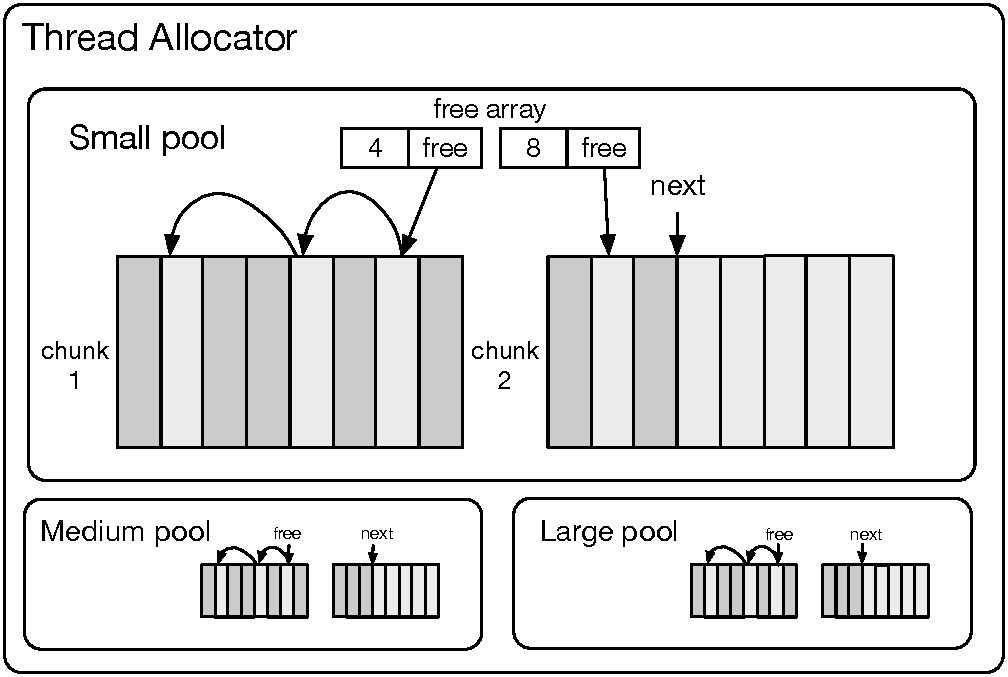
\includegraphics[width=0.7\linewidth]{figures/implementation/pool.pdf}
   \end{center}

   \caption{Threaded allocator: each thread has 3 memory pools for objects and
      each pool contains a set of memory chunks. Each pool also contains an
      ordered array for storing deallocated objects of a particular size. In
      this example, the pool for small objects has an ordered array for sizes 4
      and 8, where size 4 has 3 free objects and size 8 has just 1.}

   \label{fig:implementation:pool}
\end{figure}

In order to solve these two issues, we decided to implement a memory allocator
inspired on the SLAB allocator~\cite{Bonwick-94}. SLAB allocation is a memory
management technique created in the Solaris 5.4 kernel used for efficiently
allocate kernel objects. Its advantages include reduced fragmentation and
improved reuse of deallocated data structures since these are reused in newer
allocations.

We pre-allocate three pools of memory chunks: one pool for small objects (at
most 128 B), one pool for medium objects (at least 1 KB) and another pool for
large objects (more than 1 KB).  A memory pool is composed of multiple chunks
(or \emph{arenas}) which are large contiguous areas of memory. Each pool has a
\code{next} pointer that points to a position in the latest chunk where objects
have not been allocated yet. The third and final element of the memory pool is
the \code{free array}, which is an array which is ordered by size and each
position points to a free object of a given size. To locate free objects, a
binary search is performed on the sorted array and the array position is updated
to the next available object.

When allocating a particular object, we compute the object size and use the
appropriate pool. First, we check if there are any free objects in the free list
for that particular size and if there isn't any, we use the \code{next} pointer
to rapidly allocate space on the current chunk of the memory pool.  Whenever the
\code{next} pointer reaches the end of the latest chunk, a bigger chunk is
allocated and \code{next} is reset to the first position of the new chunk. The
objects in \code{free} list are chained together so that it is possible to mark
multiple objects as being deallocated.  An example is presented in
Fig.~\ref{fig:implementation:pool}.


In order to reduce thread contention in the allocator, each thread uses a
separate instance of the threaded allocator. When a thread wants to allocate an
object, it asks its own allocator for a new object. When deallocating, a thread
may deallocate an object that is part of another thread's chunk. However, this is
not an issue since chunks are not garbage collected from the system, which
allows another thread to efficiently reuse the pointer for a later allocation.

Our threaded allocator does not attempt to place facts of the same node physically
together. When deriving rules, this may become an issue since the thread may
need to read multiple chunks which were allocated by different threads,
increasing the number of cache line misses. In
Section~\ref{section:implementation:alternative_allocator}, we explore an
alternative allocator design and compare it against the allocator presented in
this section.
